\documentclass{article}
\usepackage{graphicx}
\usepackage{amsmath,amsthm} 
\usepackage{amsfonts} 
\usepackage{pdfpages}
\usepackage{listings}
\lstset{breaklines} 

\begin{document}

\title{COMP3331 Lab2}
\author{Ruofei HUANG}

\maketitle

\section{Exercise 1}

\subsection{Question 1}

The max congestion window size is 100, the congestion window size is back to 1
because it dectected a package loss. It has set the ssthresh to half of 100 which is 50 and start another 'slow-start' stage. \\
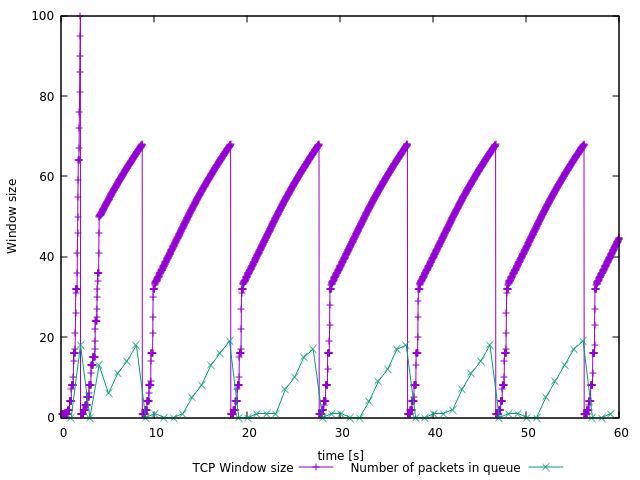
\includegraphics[width=\textwidth]{ex1q1.png}

\subsection{Question 2}

The average throught put is 188.98 packets/sec, the average throught is (500-20-20) * 188.98 = 86930.8 (Byte/sec) \\
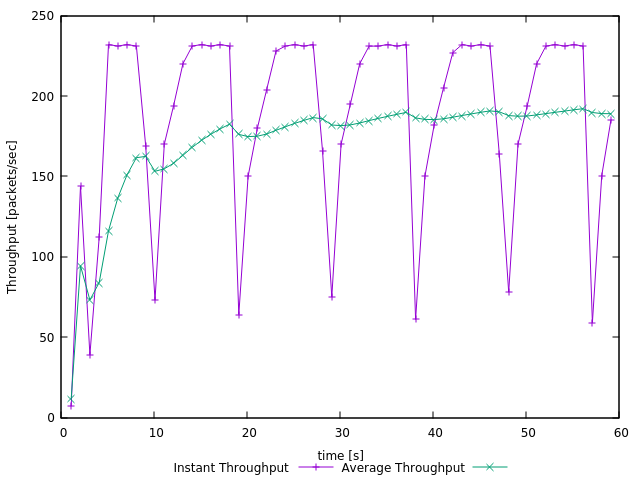
\includegraphics[width=\textwidth]{ex1q2.png}

\subsection{Question 3}

The is response this as the max window size go down till some point (around 60), there's only one oscillating from the stage of 'slow start'. If the number is lower than 50, the grap will not contain any oscillating. For the number larger than ~60, the curve is pretty much same, which means there will be package loss and has many oscillating in the graph. \\
The maximun window size to avoid oscillating is 50. The maximun throught is 227.8 packets/sec which is 113900 Bytes/sec (include header). The link capacity is 125000 Bytes, so it use 91.12\% of the link capacity.\\
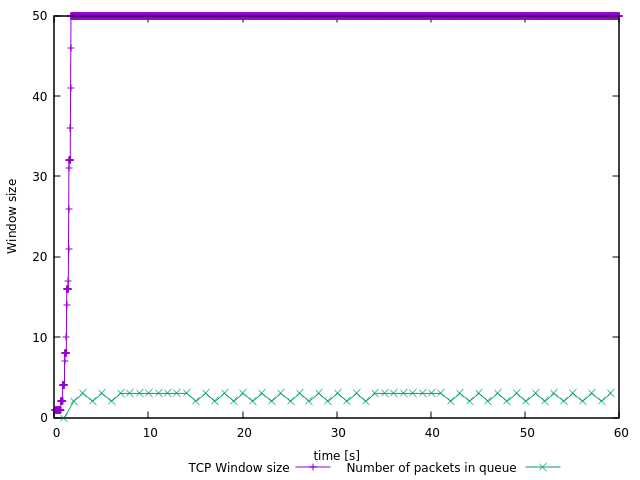
\includegraphics[width=\textwidth]{ex1q3-1.png}
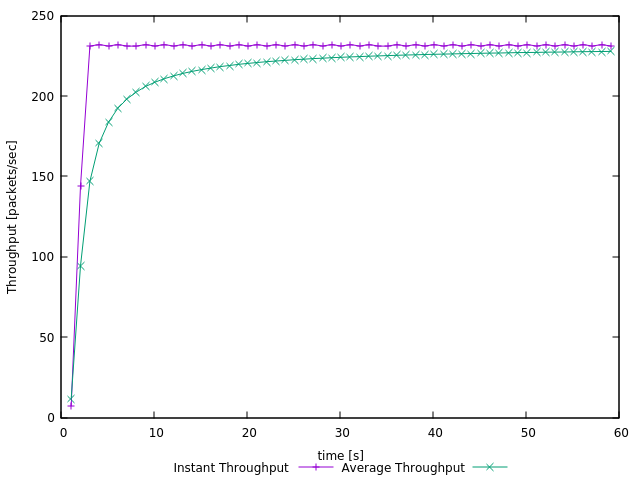
\includegraphics[width=\textwidth]{ex1q3-2.png}

\subsection{Question 4}

The window size is only get to zero once after the 'slow-start' stage compare to the Tahoe. We can see a more stable average throught in Reno implementation. The average throught for Reno is 203 package/sec while the Tahoe is 188.98 which increase a lot. \\
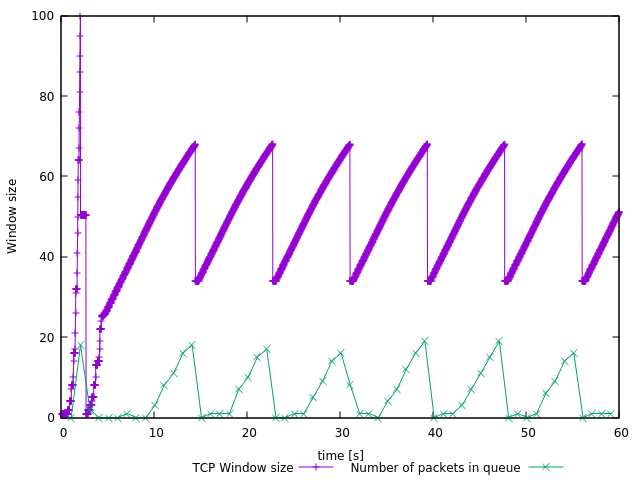
\includegraphics[width=\textwidth]{ex1q4-1.png}
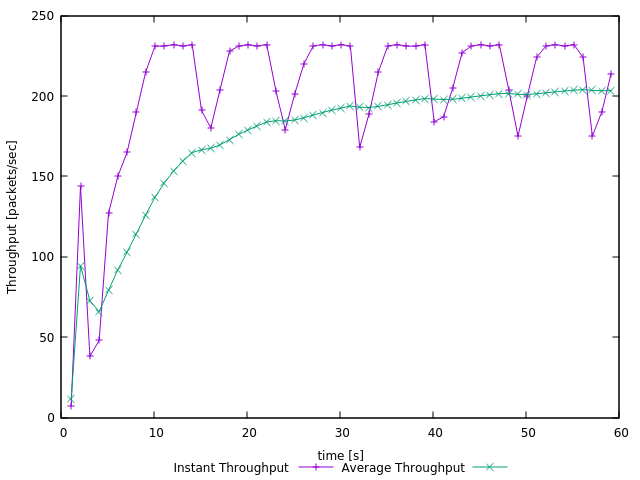
\includegraphics[width=\textwidth]{ex1q4-2.png}
\section{Exercise 2}

Not included.

\section{Exercise 3}

\subsection{Question 1}

TCP have flow control, it will have oscillating due to congestion control mechanism. On the other hand, the UDP can use all the capacity at start of  transmit. Yes I can, the red one.\\
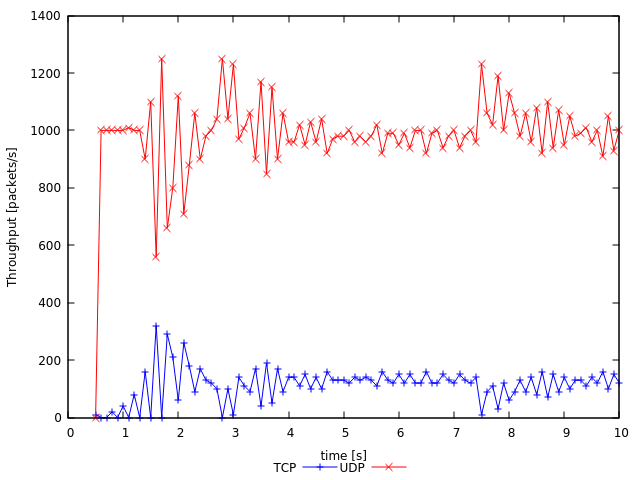
\includegraphics[width=\textwidth]{ex3q1.png}

\subsection{Question 2}
\begin{itemize}
\item UDP doesn't need to wait for ACK package.
\item UDP doesn't have flow control mechanism.
\item UDP doesn't care about the package is loss or corrupted, that's user level's stuff. 
\end{itemize}

\subsection{Question 3}

Advantages :
\begin{itemize}
    \item Full Speed
    \item Basic checksum for package corruption
    \item No connection is set up
\end{itemize}
Disadvantage:
\begin{itemize}
    \item Doesn't have congestion control
    \item Couldn't aware of the package loss during transmit
\end{itemize}

When the network have two people transfer the file, it will have a lot of package loss in the router, which will hurt the performance and make the central network congested. Also these droped packets are hard to be detected while doing the transmit, so the file may be both corrupted. 

\end{document}